\chapter{Virtuelle Private Netzwerke}

Der Zugriff aus der Ferne auf das lokale Firmennetzwerk ist für verschiedene Anwendungsszenarien unabdingbar. Die Vernetzung von Firmenstandorten, der Zugriff von mobilen Mitarbeitern auf das Firmennetz oder auch ein Zugang für Geschäftspartner auf das Intranet des Unternehmens müssen sicher Umgesetzt werden.
Die Technologie, die dies ermöglichen soll ist \emph{VPN}. Ein VPN ist ein virtuelles privates Netz, eine logische Verbindung die auf einem anderen, physischen Netz aufgebaut wird \cite{zisler2018computer}. Grundsätzlich eignet sich jedes Netz, hier wird jedoch nur die Verwirklichung von VPN über das Internet betrachtet. Es wird unter anderem wird zwischen folgenden Varianten unterschieden:
\begin{itemize}
  \item Site-to-Site/ Branch Office VPN: Verbindung von verschiedenen Firmenstandorten,
  \item End-to-Site/ Remote Access VPN: Verbindung eines Heimarbeitsplatzes oder eines Mobilen Mitarbeiters it dem Intranet des Unternehmens.
  \item End-toEnd VPN: Verbindung zweier Endgeräte,
  \item Extranet VPN: gewährt einem Geschäftspartner/Kunden/Lieferanten Zugang zu Teilen des Internen Netzes 
\end{itemize}

Die Umsetzung des VPN kann entweder bei einem Dienstleister eingekauft werden, dies nennt sich \emph{Trusted VPN}, oder selber als \emph{secure VPN} aufgebaut werden. Beim Einsatz von Trusted VPN sollten vertrauliche Daten zusätzlich auf Anwendungsebene verschlüsselt werden, um sie zum Beispiel vor Innentätern des Dienstleisters zu schützen. 
 Es gibt außerdem Zwischenformen, so dass nur Teile der Technologie bei einem Dienstleister eingekauft werden.


\section{Funktionsweise}

Die Basistechnologie die einem VPN zugrunde liegt ist das \emph{Tunneling}. Es handelt sich um ein Verfahren, welches  Netzwerkprotokolle in beliebige andere Netzwerkprotokolle kapselt (\emph{encapsulation}), über ein Netzwerk verschickt und an einem gegebenen Endpunkt wieder auspackt (\emph{decapsulation}). Das Tunneling kann auf verschiedenen Schichten des Protokollstapels (vergl. Anhang \ref{A1}) ansetzten. Das Prinzip des Tunneling ist in Abbildung \ref{tunnel} dargestellt. Während der Übertragung durch das Internet ist für die Weiterleitung der Datenpakete nicht relevant, dass es sich um Pakete eines virtuellen Netzwerks handelt, hier werden nur die Header X und Y ausgewertet. Die Header A und B sind für den Transport außerhalb der Endpunkte des VPNs zu verwenden. Der Header de Tunneling-Protokolls gibt dem Empfänger am Endpunkt des Tunnels Informationen darüber, wie das Paket weiterzuleiten ist. 

\begin{figure}[h]
	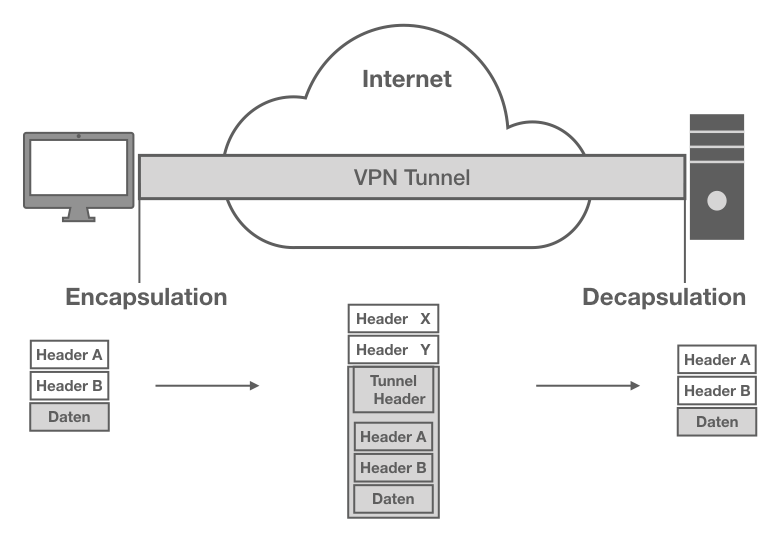
\includegraphics[width=\linewidth]{tunneling}
	\caption{Grundprinzip des Tunneling}
	\label{tunnel}
\end{figure}

 Im Folgenden sollen die wichtigsten standardisierten  Tunneling Protokolle zur VPN-Realisierung vorgestellt werden

\subsection{Layer-2-Protokolle}

\subsubsection{Layer 2 Tunneling Protocol (L2TP)}
Das L2TP ist der Nachfolger der Tunneling Protokolle PPTP (Point-to-Poit-Tunneling-Protokol) und L2F (Layer-two-Forwarding) \cite{isi-vpn}. Es kapselt Daten in PPP (Point-to-Point-Protocol \footnote{spezifiziert in RFC 1661: https://www.rfc-editor.org/rfc/rfc1661.txt}) Rahmen, ein Ende-zu-Ende Protokoll auf der Vermittlungsschicht, somit ist es möglich auch nicht-IP Pakete über das Internet zu transportieren \cite{gokulakrishnan2014survey}. Zur Authentisierung dienen die Protokolle EAP (Extensible Authentication Protocol) und CHAP (Challenge Handshake Protocol).
Da weder L2TP noch PPP die Vertraulichkeit der Daten gewähren, muss die Kommunikation zusätzlich mit IPSec (siehe Abschnitt \ref{subsub:L3}) abgesichert werden.   

\subsection{Layer-3-Protokolle}
\subsubsection{IPSec}
\label{subsub:L3}
\section{Architektur}
Das VPN-Gateway kann an verschieden Stellen an das Netzwerk angeschlossen werden. Zu beachten ist

\begin{figure}[h]
	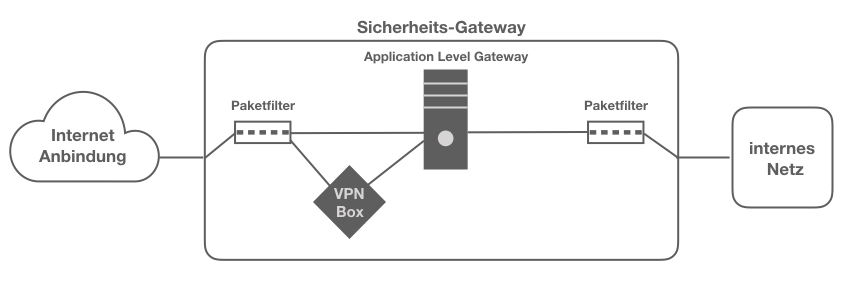
\includegraphics[width=\linewidth]{vpnarchitektur.jpeg}
	\caption{Sichere Einbindung eines VPN-Gateways in eine P-A-P Struktur}
	\label{vpnarch}
\end{figure}



\section{Anwendungsbereiche in privaten Haushalten}

Virtuelle private Netzwerke werden auch im privaten Bereich  verwendet. Hier gibt es hauptsächlich zwei Anwendungsszenarien: der Zugriff aus der Ferne auf das Heimnetzwerk zur Bedienung des IoT (Internet of Things) oder der Zugriff auf die NAS als Cloud-Alternative oder






